\documentclass[12pt]{article}

\usepackage{sbc-template}
\usepackage{graphicx,url}
\usepackage[utf8]{inputenc}
\usepackage[brazil]{babel}

\sloppy

\title{(?): UM AMBIENTE DE TECNOLOGIAS DE APOIO PARA O ENSINO DE LÓGICA DE PROGRAMAÇÃO}

\author{}

\address{}

\begin{document} 

\maketitle

\begin{abstract}
This article presents a scientific extension of the work $\textit{(?)}$, which deals with a tool for students with 
difficulties in learning of programming logic through resources based on logical structures blocks that facilitate the learning of the inherent concepts of initial subject of the Integrated Technical Computer course of $\textit{(?)}$. The application is being developed on the web platform and will consist in visual programming based on programming blocks, flowcharts and cognitive domain applications of the Revised Bloom Taxonomy in a future gamification in order to stimulate the assimilation of the logic concepts. The prototype was applied to first secondary year students of $\textit{(?)}$ in order to gather information on the ease of use and identification of the block structures used in the program. The preliminary results show that software meets the proposal to be simple and practical.
\end{abstract}
     
\begin{resumo}
Este artigo apresenta uma extensão científica do trabalho $\textit{(?)}$, que trata de uma ferramenta para estudantes com dificuldades no aprendizado de lógica de programação por meio de recursos gráficos baseados em blocos de estruturas lógicas que facilitam o aprendizado dos conceitos inerentes à disciplina inicial do curso Técnico Integrado em Informática do $\textit{(?)}$. A aplicação está sendo desenvolvida na plataforma web e consistirá na programação visual com base em blocos de programação, fluxogramas e na aplicação do domínio cognitivo da Taxonomia de Bloom Revisada em uma futura gamificação a fim de estimular a assimilação dos conceitos da lógica.  O protótipo foi aplicado para alunos do primeiro ano do ensino médio do $\textit{(?)}$ com o intuito de recolher informações no quesito facilidade de uso e identificação das estruturas de bloco utilizadas no programa. Os resultados preliminares mostram que o software atende a proposta de ser simples e prático.  
\end{resumo}

\section{Introdução} 
As dificuldades que inviabilizam a compreensão da programação variam desde a abordagem utilizada para o ensino até o problema na natureza cognitiva do aluno. Segundo \cite{GOMES:2008}, dentre os possíveis fatores deste problema destacam-se o elevado nível de abstração da programação e a falta de motivação do próprio aluno. 
\par Em um estudo de caso baseado na Taxonomia de Bloom e no Scratch, realizado por \cite{ARAUJO:2013}, percebeu-se a necessidade de incentivo ao aprendizado e do uso de outros recursos visuais como base metodológica. Portanto, modificações na abordagem utilizada durante as aulas de lógica podem torná-las mais interativas e despertarem gradativamente o interesse do aluno, apesar das possíveis dificuldades enfrentadas $(?)$.
\par O \textit{software} $(?)$ desenvolvido por $(?)$ dispõe de um ambiente de programação visual baseado em blocos e desenvolvido em Java Swing para ser empregado no aprendizado de lógica de programação, veja Figura~\ref{fig1}. Este \textit{software} apresenta limitações, como: apenas é executado localmente em uma máquina (requer \textit{download} do programa), converte o algoritmo apenas para a linguagem C e para a utilizada pelo Arduino e, além da má organização dos blocos, apresenta uma interface confusa e pouco atrativa. Objetiva-se neste trabalho uma nova fase de desenvolvimento voltada para a plataforma \textit{web}, com conversão para multilinguagens e com a implementação de novas tecnologias que ampliem as funcionalidades para o público-alvo.
	\begin{figure}[h]
		\centering
		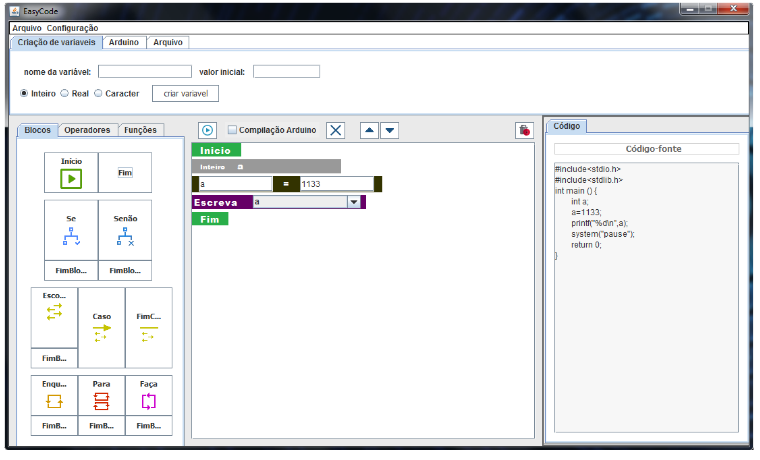
\includegraphics[scale=0.4]{2017.png}
		\caption{\textit{Layout} da tela principal do ambiente $\textbf{(?)}$.}
		\label{fig1}
	\end{figure}
	
\section{Metodologia} 
Utilizar-se-á o domínio cognitivo da Taxonomia de Bloom Revisada, que consiste nas categorias lembrar, entender, aplicar, analisar, avaliar e criar \cite{ANDERSON:2001} como atividades que o aluno deve realizar para que seja possível identificar o seu nível de aprendizado na disciplina de lógica para permitir a integração de abordagens de ensino que se adequem aos tipos de aprendizagem. Esta será a base metodológica para a gamificação que será implementada na aplicação, que contará com uma sessão de desafios onde o discente poderá revisar o conteúdo de lógica de programação (inicialmente as estruturas lógicas), codificar e gerar fluxogramas ou a montagem de blocos (veja Figura~\ref{fig2}), testar os códigos produzidos e avaliá-los, além de produzir e planejar técnicas de resoluções diversas.
\par Ademais, a taxonomia em conjunto com pesquisas quanti-qualitativas serão aplicadas para alunos do primeiro ano do ensino médio técnico em informática do $(?)$ para avaliar o nível de desenvoltura na resolução de problemas computacionais a partir do \textit{software} $(?)$.
\par Como ferramentas de desenvolvimento do \textit{website} estão sendo aplicados os \textit{frameworks} Maven, Hibernate e Bootstrap; as bibliotecas JQuery e Blockly; o padrão de arquitetura MVC; a metodologia ágil SCRUM; o controle de versão pelo GitHub; e a API JDBC. No \textit{front-end}, além do Bootstrap, utiliza-se a linguagem HTML5, JavaScript e as folhas de estilo em CSS3. O padrão XML está voltado para armazenar os blocos de programação, os processos de fluxogramas e o código-fonte gerado pela interação entre usuário e \textit{software}. 

	\begin{figure}[h]
		\centering
		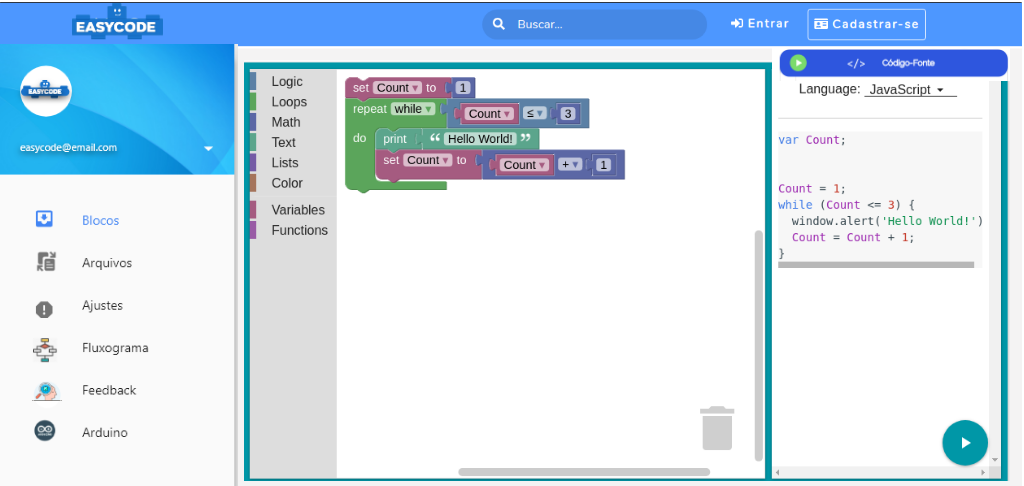
\includegraphics[scale=0.3]{bloc.png}
		\caption{Protótipo da tela de montagem de blocos do $(?)$.}
		\label{fig2}
	\end{figure}

\section{Resultados Parciais e Discussão}
O protótipo apresentado na Figura~\ref{fig2} foi disponibilizado em um questionário e posteriormente aplicado para alunos do primeiro ano do curso Técnico Integrado em Informática do $(?)$.
	\begin{figure}[!htbp]
		\centering
		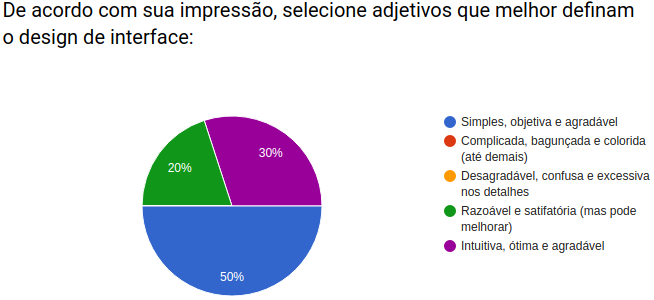
\includegraphics[scale=0.4]{g1.png}
		\caption{Gráfico relacionado ao \textit{design}.}
		\label{fig3}
	\end{figure}
\par Os resultados coletados e explicitados nos gráficos mostrados denotam que, no primeiro momento, os discentes avaliaram a \textit{interface} do \textit{software} (Veja Figura~\ref{fig3}) e a organização dos blocos de programação (Veja Figura~\ref{fig4}). Posteriormente, os alunos fizeram comentários a respeito do protótipo, tais como: ``Muito bom, fácil de compreender'' e ``Muito interessante, me agradou bastante''. Sugeriram a implementação de um \textit{chat} com a turma e apoiaram a ideia da gamificação com base em exercícios de lógica de programação.
	\begin{figure}[!htbp]
		\centering
		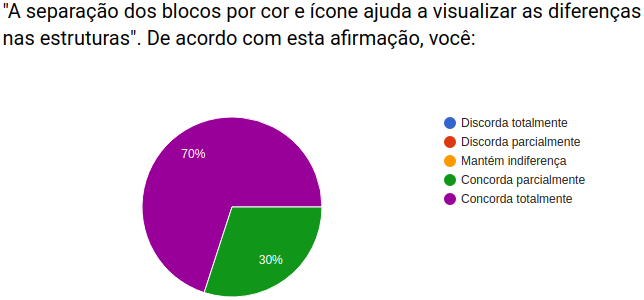
\includegraphics[scale=0.4]{g2.png}
		\caption{Gráfico em relação à organização dos blocos.}
		\label{fig4}
	\end{figure} 
\par As avaliações positivas dos alunos quanto ao protótipo demonstram que os mesmos estão aptos ao uso de novas metodologias de ensino dentro da sala de aula. Com esta expectativa, o \textit{software} proposto pode corroborar com o incentivo ao aprendizado de lógica de programação, pois a ferramenta visa atender os requisitos da nova geração de interação usuário-computador. 	

\section{Considerações Parciais}
O \textit{software} proposto é um ambiente que promove os recursos da programação para permitir que alunos com dificuldades em compreender a lógica de programação possam aprender a programar de maneira mais prática. Espera-se que as mudanças propostas colaborem com o processo de ensino-aprendizagem, permitindo que professores possam demonstrar de forma mais lúdica os conceitos da programação, por exemplo, possibilitando que os alunos compreendam as estruturas lógicas da disciplina.
\par A visualização por meio de fluxogramas dos passos para se construir o algoritmo permitirá o entendimento da aplicação da codificação de maneira simples. A implantação da conversão entre multilinguagens de programação e da biblioteca Blockly da Google permitirá que a ferramenta se torne mais atrativa para qualquer estudante. 
\par Optou-se a utilização da plataforma \textit{web} devido à maior abrangência de uso do \textit{software}, pois sem a limitação \textit{desktop} haverá disponibilidade de acesso através de qualquer dispositivo móvel com acesso à internet. Além disso, os blocos visuais e os processos dos fluxogramas servem como uma alternativa para instigar o aluno a associar a lógica ao código-fonte para várias linguagens de programação. 
\par Os próximos passos no andamento do trabalho são a implementação de recursos para a montagem de fluxogramas e, para permitir o engajamento do aluno e fomentar o uso da ferramenta, gamificação baseada em competições, além da disponibilidade de criação de perfil para o acompanhamento do progresso do aluno. Também serão feitos testes com a aplicação em sala de aula com o intuito de avaliar a desenvoltura do aluno na resolução de problemas lógicos, o qual será feito por meio de um preenchimento de um questionário específico realizado após as aulas práticas em que os alunos interagem com a ferramenta.

\bibliographystyle{sbc}
\bibliography{ArtigoEC}

\end{document}